\section{Pontos notáveis}\label{sec:pontnot}

Para melhor situar os resultados da pesquisa serão expostos a seguir alguns \textit{pontos notáveis} da freguesia, acompanhados sempre que possível de fotos, agrupados em três categorias: \textit{naturais}, \textit{religiosos} e \textit{civis}. O mapa da \autoref{fig:2019-pontosnotaveis} (p. \pageref{fig:2019-pontosnotaveis}) agrupa todos os pontos notáveis, e também algumas localidades, num só plano; recomenda-se recorrer a ele sempre que se fizer necessário situar determinado ponto ou localidade.

\subsection{Naturais}\label{subsec:pontnat}

Os principais pontos notáveis da freguesia são cursos e espelhos d'água, que formam os vales e cumeadas distintivos das muitas áreas em que ela se subdivide.

O \textit{Dique do Tororó} não é propriamente parte da freguesia; é uma de suas fronteiras, pois os limites da freguesia o margeiam. A lagoa que hoje conhecemos como o dique já foi muito maior, havendo quem afirme ter chegado a seis quilômetros de extensão antes do aterro de 1810 criar a ligação, por meio da atual ladeira dos Galés, entre as freguesias de Brotas e Sant'Anna \cite[p.~48]{santos_aguas_2010}. Um eventual historiador, também personagem histórico de destaque a quem se poderá encontrar novamente no curso desta dissertação, circunscreveu os antigos limites do dique:

\begin{citacao}
Foi formado de um lago que existia, e das aguas que nascem nas baixas do quintal do Convento de S. Bento, origem do regato denominado --- Rio das Tripas ---. sendo engrossado pelas de differentes brejos, onde fizeram-se diversas represas com paredões de terra.

Uma dessas represas era na baixa do Convento do Carmo, com a qual se retinham as aguas de alguns lagos que por ali havia, até o sitio conhecido naquelle tempo por --- \textit{Quinta do Maciel}, no qual se abriram as duas ruas, denominadas hoje de Maciel de cima e Maciel de baixo.

Outra represa era nos brejos do Convento de S. Francisco, onde entulharam um estreito que havia entre a rua de S. Miguel e a ladeira da Poeira.

A terceira represa ficava nas baixas do quintal do convento de S. Bento, com entulho entre a ladeira da Palma e da Praça, no sitio conhecido por largo do Guadelupe, actualmente Praça dos Veteranos da Independencia.

Encaminhadas todas essas aguas formaram o grande fóco aquatico, a que deram o nome de \textit{Dique}, que quer dizer \textit{aguas retidas}, visto que fez-se tambem um forte paredão de terra, que ainda serve de represa [\textit{em 1885}], com um sangradouro por onde se esgotam as aguas que formam o Rio Lucaia, o qual vai ter ao Rio Vermelho \cite[pp.~393-394]{amaral_resumo_2013}. 
\end{citacao}

Um comentador deste texto ressalta, a respeito dos ``brejos'' que engrossaram a vazão rumo ao dique:

\begin{citacao}
Esses brejos tiveram as seguintes denominações, antes da primeira invasão hollandesa: \textit{dique dos Sapateiros}, na baixa do mesmo nome, o qual se communicava com o \textit{brejo do Quibungo}, formado pelas aguas da fonte de igual nome, ao Maciel de Baixo, entre a ladeira da Saúde e o largo de S. Miguel; \textit{brejo do João de Mattos}, entre a baixa da ladeira da O. 3ª de S. Francisco e a praça Guadalupe. Outros, pantanos e aguada s se seguiam ao brejo de João de Mattos até a baixada da antiga horta do mosteiro de S. Bento \cite[pp.~393-394]{amaral_resumo_2013}.
\end{citacao}

O dique hoje é alimentado principalmente por esgotos dos bairros circunvizinhos \cite[p.~41]{santos_aguas_2010}.

O rio \textit{Camarajipe}, \textit{Camaragipe} ou \textit{Camorogipe}\footnote{A grafia muda de acordo com a documentação encontrada; salvo quando constar na fonte original, será adotada a grafia ``Camarajipe'' sugerida por \citeonline{edelweiss_camarajipe_1969}.}, centro da terceira maior bacia hidrográfica de Salvador na atualidade\footnote{A maior é a do rio \textit{Ipitanga}, sub-bacia do rio \textit{Joanes} \cite[p.~311]{santos_aguas_2010}, seguida pela do rio \textit{Jaguaribe} \cite[p.~229]{santos_aguas_2010}.}, nasce longe de Brotas, nas cercanias do dique do Cabrito, recebe o afluxo de muitos afluentes --- como o \textit{rio Azacá}, no Calabetão --- e corta longitudinalmente o território soteropolitano até desembocar no Atlântico. O Camarajipe teve seu curso alterado na década de 1970 para evitar as constantes enchentes nas áreas mais baixas do Rio Vermelho; por meio de dragagem e rebaixamento do substrato do vale, seu curso foi estendido até o vale do \textit{rio Pernambués}\footnote{O mapa da \citeonline{salvador_mapa_1969} ainda permite ver o rio Pernambués como um curso d'água sem nome que nasce entre o quartel do 19º Batalhão de Caçadores e o ``beco do Francelino'' (atual rua Nossa Senhora do Resgate), recebe o afluxo de alguns pequenos tributários e segue até encontrar o Camarajipe no ``Hipódromo'' (atual Salvador Shopping). O rio ainda existe --- quase um córrego que flui rente à atual avenida Luiz Eduardo Magalhães.}, de onde foi possível canalizá-lo até sua foz atual, no bairro do Costa Azul.

Dentro da bacia do Camarajipe destacam-se quatro afluentes de extrema importância vistos no mapa de \citeonline{weyll_mappa_1851}; ainda que de curso mais curto, mais estreitos e de menor vazão que seu rio principal, sua importância está na demarcação de vales e cumeadas da freguesia. Em primeiro lugar, o \textit{rio das Tripas}, vizinho ao qual corria a rua da Vala, no trecho correspondente à atual avenida Heitor Dias; ele escava o vale que separa a freguesia de Brotas da freguesia do Santo Antônio. O segundo rio é indicado por \citeauthoronline{weyll_mappa_1851} como sendo o \textit{Santo Antônio}, hoje um esgoto que corre quase paralelamente à atual rua do Baixão, no Matatu \cite[p.~136]{santos_aguas_2010}; ele escava o vale que separa as cumeadas do Matatu Grande e do Matatu Pequeno. O terceiro rio é o \textit{Córrego das Beatas}, correspondente, grosso modo, à atual Baixa do Matatu, também transformado em esgoto \cite[p.~158]{santos_aguas_2010}; ele separa o Matatu Grande e a Quinta das Beatas por um vale. O Córrego das Beatas é afluente do rio \textit{Bonocô} ou \textit{Campinas}, que no mapa de \citeonline{weyll_mappa_1851} separa a Quinta das Beatas da cumeada cortada pela Estrada de Brotas e hoje corre sob a avenida Mário Leal Ferreira (popularmente conhecida pelo mesmo nome do rio).

O rio \textit{Lucaia}\footnote{Certa etimologia duvidosa e de curso fácil --- que confunde \textit{Lucaia} com \textit{Lucas}, \textit{Lucano} ou \textit{Lucania}, coisa que etimólogos desautorizam \cite{guerios_nomes_1981} --- diz significar \textit{Lucaia} algo como ``luminoso, brilhante'' em latim. Uma etimologia decerto mais erudita apresenta duas alternativas. Na primeira, o rio teria sido originalmente chamado de rio da \textit{Leocádia}, nome que com o tempo foi sendo transformado em \textit{Lucaia}. Na segunda, aliás mais plausível, os habitantes originais da terra que veio a formar Salvador teriam chamado o rio de \textit{Urucaya}, palavra tupi cujo significado não foi possível localizar; ``pelo abrandamento ou assimilação do \textit{r} em \textit{l}, quando pronunciada a palavra pelos africanos, se transmudou o nome em \textit{Ulucaia} e finalmente, pela queda da vogal inicial, ficou \textit{Lucaia}'' \cite[p.~68]{amaral_resumo_2013}.} corta o vale que separa o Engenho Velho de Brotas do Engenho Velho da Federação. Descrito conforme indicam \citeonline{santos_aguas_2010} e \citeonline{weyll_mappa_1851}, nasce nas encostas e grotões da cumeada onde hoje se localiza a avenida Joana Angélica; recebe inicialmente contribuição do dique do Tororó e do \textit{rio de São Pedro}, que escava o vale onde hoje se localiza a avenida Reitor Miguel Calmon, no Canela; era alimentado mais adiante por um riacho que escavou o atual Vale da Muriçoca e por outro que escavou o Vale do Ogunjá, um desembocando em frente ao outro; recebia mais à frente as águas do rio que escavou o vale onde hoje se situa o Hospital Geral do Estado da Bahia; e desemboca no largo da Mariquita (Rio Vermelho), onde se localizava a foz do rio Camarajipe antes de sua transposição nos anos 1970.

A última bacia hidrográfica a atravessar o distrito de Brotas importa quase apenas por ser um de seus limites naturais: é o \textit{rio das Pedras}, cuja bacia é atualmente a quarta maior do município e inclui a sub-bacia do rio \textit{Pituaçu} \cite[p.~175]{santos_aguas_2010}, também tido em alguns documentos como um dos limites da freguesia. Este rio tem leito de curta extensão, pois trata-se de um curso d'água formado pela fusão dos rios \textit{Cascão}, \textit{Saboeiro}, \textit{Cachoeirinha} (incluindo os rios \textit{Orifugi} e \textit{Bitifilim / Campo Seco} que nele deságuam) e Pituaçu, estes, sim, de maior extensão. Sua foz é na Boca do Rio, no lugar onde se situava a antiga sede de praia do Esporte Clube Bahia \cite[p.~175]{santos_aguas_2010}. Um mapa municipal de 1969 \cite{salvador_mapa_1969} (cf. reprodução em menor resolução no \autoref{anexo-mapas}, p. \pageref{fig:1969-mapaprefeitura}) permite visualizar a bacia do rio das Pedras e do rio Pituaçu, ainda que o curso dos rios houvesse sido ligeiramente alterado muito antes da produção deste mapa pela construção do sistema de abastecimento de água de Theodoro Sampaio, que construiu represas em todos os rios da bacia. Visualiza-se neste mapa as bacias do Pituaçu e do rio das Pedras com uma nitidez que mapas posteriores não mais permitiram, por força da ocupação maciça do entorno dos rios e sua transformação em canais de esgoto.

Neste mapa de 1969 também é possível localizar, ainda que não esteja nomeado, o \textit{riacho da Estiva}, ausente do mais completo estudo das bacias hidrográficas soteropolitanas a ser publicado até o momento \cite{santos_aguas_2010}\footnote{O estudo de \citeonline{santos_aguas_2010}, com todo o respeito ao grande e pioneiro trabalho de síntese que representa, pecou por não haver consultado mapas históricos que indicam o nome de cursos d'água infelizmente perdidos na memória dos soteropolitanos. Além do riacho da Estiva, em outra oportunidade foi possível observar como neste mesmo estudo foi simplesmente suprimida a existência do \textit{rio Camarão}, que aparece no mapa de \citeonline{lealteixeira_carta_1830} com nome e tudo, e no mapa de \citeonline{weyll_mappa_1851} foi representado, embora sem nome, com um curso muito mais bem delineado a partir de suas nascentes no fundo do cemitério do Campo Santo. No estudo, a bacia hidrográfica do rio Camarão foi infelizmente substituída pela ``bacia hidrográfica de Ondina'', sem qualquer referência ao antigo nome do rio. O rio Camarão foi ``identificado'' no estudo, sem qualquer menção a seu antigo nome, como ``um curso d’água completamente degradado no seu escoamento superficial, que corre paralelo à Rua Nova do Calabar, em áreas bastante impermeabilizadas, ao fundo dos lotes lindeiros a esta via'' \citeonline[p.~31]{santos_aguas_2010}. Este rio tem história profundamente ligada à \textit{fazenda Camarão} que existiu na área por onde corre, e história ainda mais interessante pelo fato de moradores e lideranças comunitárias do Calabar situarem sua ancestralidade tanto nos \textit{kalabari} (grupo étnico dos \textit{ijaw} da Nigéria) quanto nos \textit{bantu} e \textit{fula} justafluviais ao Wouri, rio na África Ocidental a que os portugueses desde 1472 chamavam de ``rio dos Camarões'' e que terminou por dar nome à atual República dos Camarões. No que diz respeito a outras fontes e minadouros encontrados na mesma ``bacia'', o mapa de \citeonline{weyll_mappa_1851} indica outros dois cursos d'água: um que parece ter escavado o vale por onde hoje situa-se a avenida Adhemar de Barros, em Ondina, e outro que corta um vale por onde talvez passe hoje a avenida Anita Garibaldi, atravessa a vila Matos e desemboca no ponto onde o alto da Sereia encontra-se com a praia da Paciência, no Rio Vermelho. É evidente que num estudo de grande porte e amplo escopo falhas como esta seriam inevitáveis, ainda mais quando a pesquisa em fontes foi secundarizada em função da caracterização ambiental e da qualidade das águas das bacias hidrográficas soteropolitanas, mas o reparo é necessário para que estes e outros equívocos não deslustrem o mérito do trabalho.} mas identificado no mapa de \citeonline{lealteixeira_carta_1830} (cf. \autoref{fig:1830-lealteixeira}, p. \pageref{fig:1830-lealteixeira}); trata-se, no mapa municipal de 1969, do tênue fio d'água iniciado no ``Campo Sêco'' que atravessa a avenida ``governador Luiz Viana Filho'' para desaguar no rio das Pedras, em frente ao ``Bate Facho''. Provavelmente este rio está hoje soterrado pela avenida Edgard Santos em seu curso principal e pela rua das Embuias num braço que a ele afluía.

\subsection{Religiosos}\label{subsec:pontrel}

\afterpage{
\begin{figure}[!htp]
\caption{Igreja de Nossa Senhora de Brotas em sua configuração atual.}
\begin{subfigure}[b]{0.4\textwidth}
\centering
\includegraphics[width=\textwidth]{3-cap2/complementos/imagens/nsbrotas-fachada.jpg}
\caption{\footnotesize Fachada. \textbf{Fonte:} \url{http://www.igrejas-bahia.com}}
\label{Fachada}
\end{subfigure}
\  %espaco separador
\begin{subfigure}[b]{0.4\textwidth}
\centering
\includegraphics[width=\textwidth]{3-cap2/complementos/imagens/nsbrotas-altarmor.jpg}
\caption{\footnotesize Altar-mor. \textbf{Fonte:} \url{http://www.igrejas-bahia.com}}
\label{Altar-mor}
\end{subfigure}
\  %espaco separador
\begin{subfigure}[b]{\textwidth}
\centering
\includegraphics[width=\textwidth]{3-cap2/complementos/imagens/nsbrotas-interior.jpg}
\caption{\footnotesize Interior. \textbf{Fonte:} \url{http://www.igrejas-bahia.com}}
\label{Interior}
\end{subfigure}
\end{figure}
}

É inevitável tratar dos pontos notáveis deste distrito sem começar pela \textit{igreja de Nossa Senhora de Brotas}, cujo orago emprestou seu nome à freguesia. Não é tarefa simples, pois nem o próprio IPAC-BA, quando do tombamento da igreja pelo Decreto Estadual nº 11.673/2009, soube precisar sua data de fundação, remetendo-a, pela ``oralidade'', a 1714 \cite{ipac_brotas_2015}. Esta ``oralidade'', todavia, é controversa. 

Em primeiro lugar, a historiografia demonstra que sua construção nem foi tão rápida, nem tampouco precedeu a criação da freguesia em 1718; o mais provável é que a freguesia tenha sido criada primeiro, e o templo tenha vindo depois. As razões são muito comezinhas. Havia na paróquia ``apenas algumas fazendas e engenhos e poucos moradores, na maior parte de poucos recursos'' e, portanto, ``entravam poucas esmolas para a construção da matriz de pedra e cal'' \cite[p.~10]{ott_engenhos_1996}. Já em 1729 os paroquianos pediam ao rei João V uma ajuda de custo para a construção da igreja que viria a substituir a arruinada capela de taipa que sediava a freguesia \cite[p.~10]{ott_engenhos_1996}, e há ainda uma carta do Provedor-Mor da Fazenda Real do Estado do Brasil ao rei João V, datada de 1732, pedindo-lhe que socorresse as obras de construção do templo, vez que os paroquianos não dispunham de recursos \cite[p.~30]{vivas_botelho_2011}. Em 1739 o rei deu nove mil e quinhentos cruzados para acabar as obras da capela-mor, repartidos em pagamentos de três anos \cite[p.~10]{ott_engenhos_1996}; mesmo assim, em 1741 a Irmandade do Santíssimo Sacramento e Nossa Senhora de Brotas chegou a tomar empréstimo à Santa Casa de Misericórdia para terminar algumas obras na matriz, e tudo indica que em 1753 a obra não havia sido concluída pela falta de esmolas para continuá-la, resultando disto novo pedido de auxílio ao rei José I, que não se sabe se foi atendido \cite[p.~10]{ott_engenhos_1996}. Ora, se o templo aparentava não estar ainda concluído em 1753, malgrado os esforços hercúleos dos paroquianos, é impossível que houvesse sido fundado em 1714. 

Em segundo lugar, dois estudos antigos sobre este templo \cite{campos_brotas_1942,texbar_capellas_1930} apontam outros fatos elucidadores sobre sua construção. O mais antigo dos dois estudos diz que a igreja de Nossa Senhora de Brotas é de construção posterior à instituição da freguesia em 1718, pois sua matriz teria sido, nos primeiros tempos, a antiga igreja de São Paulo \cite[p.~344]{texbar_capellas_1930}. O segundo dos dois estudos não dá informações outras além da existência, antes de reforma já antiga, de uma campa na capela-mor onde se destacava 

\begin{citacao}
um escudo d'armas em relevo [\dots] [que] talvez lançasse alguma luz sobre a história do santuário, porque diziam os antigos moradores do `arraial' [o Largo de Brotas] que sob aquela pedra jaziam as cinzas do construtor da igreja \cite[p.~88]{campos_brotas_1942}
\end{citacao}

Como se vê, a data de início das obras do templo é incerta, estando em algum lugar entre 1714 e 1729; sua inauguração é ainda mais incerta, diante da sucessão de pedidos de auxílio para conclusão das obras. É possível que em 1757, quando do primeiro censo eclesiástico da freguesia, o templo já estivesse construído, mas a existência da data 1772 sobre o arco central da galilé põe em dúvida esta hipótese. Teria sido ela concluída ou meramente reformada em 1772? A documentação encontrada, bem como as fontes secundárias, não permitem estabelecer qualquer das duas hipóteses como definitiva; o que é possível concluir, entretanto, é que neste ano o templo chegou a um formato definitivo, sujeito a reformas posteriores, como a de abril de 1889\footnote{\textbf{Treze de Maio}, 01 abr. 1889, p. 3}. Em sua configuração atual, trata-se de uma igreja com fachada em estilo rococó e altares em estilo neoclássico. Já a Irmandade do Santíssimo Sacramento e Nossa Senhora de Brotas foi criada em 1781 \cite[p.~172]{VASCONCELOS2002}, que no último quarto do século XIX ainda era muito ativa\footnote{A pesquisa realizada nas edições do jornal \textbf{O Monitor} publicadas entre 1876 e 1881 evidenciou a atividade da irmandade durante o período, em especial na realização de funerais e missas solenes de seus integrantes}.

O mito fundador do templo diz que a devoção a Nossa Senhora de Brotas se deve ao fato de um homem muito pobre, que morava no vale atrás da atual igreja, ter apelado com sucesso à Virgem Maria para salvar do afogamento a única vaca que lhe dava sustento e à sua família; como a santa teria aparecido ao vaqueiro com seu filho ao colo nas \textit{grotas} existentes atrás do sítio da atual igreja, daí teria surgido o nome primitivo de ``Nossa Senhora das Grotas'', que sendo variado ao longo do tempo resultou na atual denominação do distrito \cite{campos_brotas_1942,texbar_capellas_1930}. A única fonte deste mito, um boletim paroquial de 1924 \cite[p.~345]{texbar_capellas_1930}, não menciona a longa cauda do mitema do apelo do vaqueiro à santa, que pode ser rastreado, passando por Juazeiro (1710), por Sergipe (1650) e pela igreja da Graça (onde se relata ter existido uma imagem de Nossa Senhora de Brotas muito antes da fundação da freguesia) \cite[p.~89-92]{campos_brotas_1942} até chegar à antiquíssima vila portuguesa de Brotas, atualmente uma freguesia do concelho de Mora, distrito de Évora, na região do Alentejo; esta vila foi fundada em torno da igreja de Nossa Senhora de Brotas, a primeira de todas, construída em 1424 \cite{campos_brotas_1942, correia_brotas_2010, portugal_brotas_2015}. A Arquidiocese de São Salvador da Bahia, inclusive, reconhece esta ``filiação'' \cite{arqui_brotas_2015}.

\begin{figure}[!htp]
\caption{Igreja do Deus Menino em sua configuração atual.}
\centering
\includegraphics[width=1\textwidth]{3-cap2/complementos/imagens/deusmenino.jpg}{\footnotesize \par \textbf{Fonte:} \url{http://www.wikimapia.org} \par}
\end{figure}

A \textit{Capela do Deus Menino} é a precursora da atual igreja homônima, situada na atual rua Brígida do Vale, no Engenho Velho de Brotas. Apesar de dar nome a uma área inteira do distrito, como visto na documentação pesquisada (Alto da Capelinha, Rua da Capelinha etc.), não foi possível encontrar nem na documentação nem na bibliografia qualquer informação acerca de sua fundação ou de sua construção.  

\begin{figure}[!htp]
\centering
\caption{Igreja do Senhor Bom Jesus dos Milagres em sua configuração atual.}
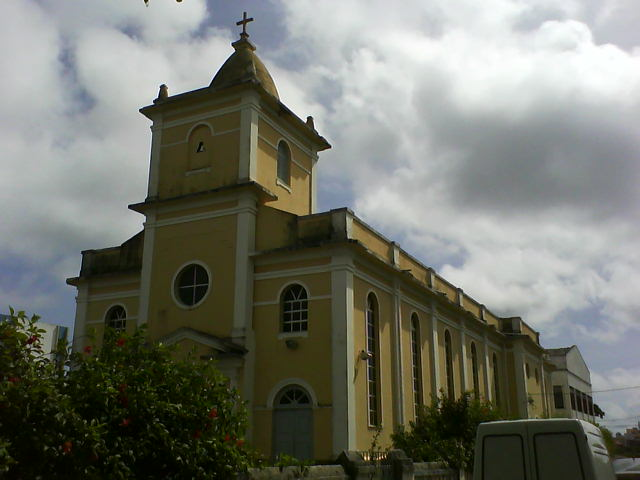
\includegraphics[width=1\textwidth]{3-cap2/complementos/imagens/bomjesusdosmilagres.jpg}{\footnotesize \par \textbf{Fonte:} \url{http://www.igrejas-bahia.com} \par}
\end{figure}

A \textit{Capela do Senhor Bom Jesus dos Milagres} é a precursora do templo homônimo existente ainda hoje no Largo dos Paranhos, na bifurcação entre o Matatu e Cosme de Farias. Pouco há de informações sobre ela, sabendo-se apenas que foi construída em 1862 \cite[p.~251]{VASCONCELOS2002} em estilo neoclássico. Sua forma atual resulta de reforma realizada em 1954. Esta capela foi associada à Irmandade de Nosso Senhor dos Milagres, que em 1873 requereu à Assembleia Legislativa da província, junto com moradores das Pitangueiras, recursos para pagar um capelão para celebrar os atos religiosos, pois era ``distante da igreja matriz cerca de meia legua''; este requerimento, analisado pelos deputados, foi julgado merecedor da atenção da Assembleia, mas sua deliberação foi condicionada aos ``recursos que ministrar o orçamento provincial'' \cite[p.~46]{bahia_relatassleg_1873}. O pedido foi posteriormente aprovado \cite[p.~53]{bahia_relatassleg_1873}. Durante todo o século XIX esta capela viveu em estado precário de conservação, sendo constantes as reclamações e as destinações de verbas para reformas; em 1864, por exemplo, a Assembleia Provincial destinou 500\$000 para sua reforma\cite[anexo~2, p.~2]{silvagomes_relatorio_1864} e em 1877 ainda outros 2:000\$000\footnote{\textbf{O Monitor}, 12 abr. 1877, p. 1}, mas em abril de 1889 encontrava-se a capela novamente em ruínas \footnote{\textbf{Treze de Maio}, 01 abr. 1889, p. 3}. 

\begin{figure}[!htp]
\centering
\caption{Igreja de Nossa Senhora da Luz em sua configuração atual.}.
\includegraphics[width=1\textwidth]{3-cap2/complementos/imagens/nsluz.jpg}{\footnotesize \par \textbf{Fonte:} \url{http://www.igrejas-bahia.com} \par}
\end{figure}

A \textit{Capela de Nossa Senhora da Luz} é a precursora da atual igreja de mesmo nome, situada na praça igualmente homônima, na Pituba. Há interessante registro histórico apresentado no \textit{website} da paróquia:

\begin{citacao}
Conforme a tradição, pelos anos de 1580, uma menina de uns doze anos de idade, andando para apanhar gravetos para cozinhar, sentindo sede, viu (ou imaginou ver) surgir entre a mata e a areia, uma figura de uma mulher linda, com um menino sentado no braço esquerdo e na mão direita uma vela acesa; atrás da figura veio um manancial de água, e todo o quadro como iluminado com uma luz azul. – Saciada a sede, correu para casa e comunicou aos seus pais o ocorrido, os quais vieram acompanhando-a; chegados ao lugar por ela indicado, constataram a existência do manancial de água, não sabendo explicar se já existia antes; e mais nada viram. Este lugar situa-se perto da confluência das ruas São Paulo com Rio Grande do Sul, bem perto da Praça Belo Horizonte.

Passados anos, a menina de então, já adulta, avistou em casa do capitão Felipe Correa uma Imagem de Nossa Senhora da Luz, trazida de Portugal, reconhecendo ser a mesma que tinha visto ou imaginado na fonte.

Pelos anos de 1600, o latifundiário e capitão Felipe Correa, proprietário da Fazenda Pituba, fez construir em terreno de sua propriedade, uma capela de taipa, no lugar que hoje seria entre as ruas Minas Gerais e Otávio Mangabeira, colocando na mesma a Imagem trazida de Portugal, de talha de madeira, medindo 53 centímetros, com o pedestal, conservada na sua Igreja da Pituba.

Durante os anos de 1610 a 1642, sendo atendente espiritual do litoral baiano, compreendido entre o Rio Vermelho e a Vila de Abrantes, o artista e religioso do Mosteiro de São Bento, Frei Agostinho da Piedade, o grande escultor e ceramista, fez para a capela da Pituba uma Imagem de Nossa Senhora da Luz, de barro cozido, e policromado, que é uma relíquia preciosa de quando o Brasil amanhecia, a qual no ano de 1949 foi restaurada, sendo reencarnada.

Os herdeiros do capitão Felipe Correa, capitão Manoel Gonçalves Saraiva e sua esposa Francisca Ferreira e o irmão desta, Francisco Ferreira, restauraram a capela pelos anos de 1663 \cite{fernandez_historia_1969}.
\end{citacao}

É preciso, entretanto, checar as informações com outras fontes para averiguar a precisão histórica do relato. Já encontramos a capela ereta em 1673, quando a Santa Casa de Misericórdia, responsável por pagar as côngruas dos sacerdotes deste templo entre 1676 e 1680, pagou também 13\$250 a Manoel Gonçalves Saraiva pelos consertos nela realizados. \cite[p.~11]{ott_engenhos_1996}. 

Vistos os principais pontos notáveis religiosos encontrados na documentação pesquisada e na bibliografia consultada, é preciso ressaltar uma lacuna seriíssima nesta classificação. Qualquer templo ou local consagrado reflete a cosmovisão daqueles que em determinada formação social assumem o papel de \textit{dominantes} e \textit{exploradores}; aos \textit{dominados} e aos \textit{explorados}, conquanto tenham cosmovisão própria, costuma caber apenas a aceitação desta cosmovisão, ou a convivência com ela. Por este ponto de vista, a naturalização das igrejas, capelas e demais edifícios sagrados de matriz cristã como únicos ou principais pontos notáveis religiosos deve ser questionada, para retirar do ocultamento os lugares e edifícios sagrados de outras religiões.

A naturalização do cristianismo como ``única'' religião praticada em Salvador (ou no Brasil, para ser mais preciso quanto a este mito) é o mais evidente resultado de uma longa tradição de \textit{repressão e ocultamento das religiões afrobrasileiras}; a repressão a tais religiões, vigente até tempos bastante próximos, operou-se por meio da destruição de templos e lugares sagrados; do roubo de objetos litúrgicos pelas autoridades policiais, para exibição como ``curiosidade antropológica''; da humilhação pública, do espancamento, da prisão e do assassinato de sacerdotes; da perseguição e discriminação a seus praticantes etc. Brotas, tal como outros distritos soteropolitanos, tem longa tradição como território construído também pelas práticas religiosas de matriz africana. Não faltam notícias de ``batuques'', ``calundus'', ``candomblés'' e ``terreiros'' por todo o território da freguesia \cite{carneiro_candomble_1954,reis_domingos_2008,REISSILVA1989}, que no século XIX registrou a maior incidência de candomblés em toda a cidade \cite[p.~60]{santana_itiner_2008}; das mais antigas, entretanto, resta pouco senão traços daquilo que um famoso antropólogo franco-brasileiro registrou como sendo um dos pontos de maior concentração de terreiros, junto à Quinta dos Lázaros, à Gomeia (atual São Caetano) e ao Rio Vermelho \cite{bastide_mystique_1978}. A perseguição resultou, entre outras coisas, na necessidade de constantes mudanças territoriais daquilo que, em outras circunstâncias, seriam assentamentos fixos em terras sagradas. O terreiro \textit{Mutá Lambô ye Kaiongo}, por exemplo, hoje situado em Cajazeiras XI, remonta suas origens familiares a outros templos que funcionaram em ``Daniel Lisboa, Bonocô, Campinas de Brotas, Cosme de Farias'' \cite[p.~50]{alves_paquetan_2010} --- todos contidos no território de Brotas. De forma parecida, o terreiro \textit{Tumba Junsara}, fundado em 1919 em Santo Amaro, foi transferido pouco depois para o Beiru, já em Salvador; por volta de 1920 funcionava na Ladeira do Pepino (antiga rua Uruguaiana), nº 70, em Brotas, e em 1938 radicou-se na 2ª Travessa da Vila América, nº 30, no Engenho Velho de Brotas \cite[p.~61]{rego_terreiros_2006}

Um exemplo, o do \textit{terreiro do Alaketo}, bastará para demonstrar as profundas ligações do território de Brotas com a prática de religiões afrobrasileiras. Assim se registrou o mito fundador deste templo:

\begin{citacao}
\dots sua fundadora foi uma princesa chamada Otampê Ojarô, originária do reino africano de Keto, que recebeu no Brasil o nome cristão de Maria do Rosário Francisca Régis. Otampê Ojarô teria sido sequestrada ainda criança, aos nove anos de idade, por soldados do exército daomeano, às margens de um rio situado nos ``fundos do reinado de Ketu'', juntamente com sua irmã gêmea, Obokô ou Bokô Mixôbi, tendo sido em seguida vendidas a traficantes, com destino à Bahia. Compradas no mercado de escravos e alforriadas aos 16 (ou 18) anos pelo próprio orixá Oxumarê, na figura de um homem branco, ``rico, alto e simpático'', teriam então voltado à África, casando-se Otampê Ojarô, aos vinte e dois anos, com um certo Babá Láji ou Oláji, nagô de Ketu de família consagrada ao orixá Oxalá.

Após o matrimônio, o casal teria voltado à Bahia com o objetivo de fundar um candomblé. Babá Láji adotou o nome de João Porfírio Régis ``pela parte do Brasil'', e arrendou, ``por seis patacas'' anuais, um terreno na antiga Estrada do Matatu Grande, ali fundando um terreiro dedicado a Oxóssi, o Alaketo, e edificando o ilê Maroiá Láji, casa de culto dedicada a Oxumarê, onde até hoje são zelosamente mantidas essas tradições religiosas. A primeira filha do casal, nascida na Bahia e chamada de Akobiodé, também viria a receber o título de Iyá e tornar-se a segunda iyalorixá da casa. Akobiodé, por sua vez, teria um filho chamado João Francisco Régis, cujo filho, José Gonçalo Francisco Régis, casou-se com Silvéria Clemente de Jesus, Sili, a qual recebeu o título de Iyá Merenundê, tornando-se a terceira iyalorixá da linhagem. Deste casal nasceu Dionísia Francisca Régis, Obá Oindá, a quarta iyalorixá do Alaketo, que morreu centenária em 1953, tia-avó e mãe-de-santo responsável pela formação da atual iyalorixá da casa, Olga do Alaketo \cite[p.~345-346]{silveira_alaketo_2003}.
\end{citacao}

Há aspectos interessantíssimos na tradição do Alaketo, a serem vistos mais detalhadamente na \autoref{subsec:matatubeatas} (p. \pageref{subsec:matatubeatas}). Como o Alaketo existiram em Brotas outros terreiros em grande número, de que hoje pouco mais resta além de traços fugidios na memória coletiva e nas tradições orais.

\subsection{Civis}\label{subsec:pontciv}

Além dos pontos notáveis naturais e religiosos, foram encontrados na documentação pesquisada e na bibliografia consultada vários pontos notáveis \textit{civis}.

O \textit{Solar Boa Vista} é o palacete com torre encontrado ainda hoje no centro do Engenho Velho de Brotas. Ao longo de sua existência teve vários usos, a maior parte deles ligada a alguma função sanitária ou administrativa da cidade.

O solar foi erguido por volta das últimas décadas do século XVIII a mando do traficante de pessoas escravizadas \textit{Manuel José Machado}, que ordenou construírem-lhe torre alta o suficiente para acompanhar a chegada de navios ao porto de Salvador \cite[p.~127]{mattos_panorama_2011}. Em 1824 \textit{Joaquina Josefa de Santana Machado} recebeu o solar como herança; em 1831 o imóvel foi vendido a \textit{Joaquim Ramos de Araújo}; e em 1858 o médico \textit{Antônio José Alves}, cirurgião e professor de patologia externa da Faculdade de Medicina e pai de \textit{Antônio de Castro Alves}, o ``poeta dos escravos'', adquiriu a propriedade e investiu grande parte de seus recursos para transformá-la em uma casa de saúde. Castro Alves, o poeta, chegou inclusive a dedicar ao solar seu poema ``A Boa Vista'', transcrito no \autoref{cap:boavista} (p. \pageref{cap:boavista}).

O intento de Antônio José Alves com a aquisição do imóvel terminou sendo cumprido: em agosto de 1869 o governo da Bahia comprou o imóvel, com base na Lei provincial nº 1.089, para a instalação de um hospital. Em 24 de junho de 1874, foi inaugurado no local o Azylo São João de Deus, com um hospital, sob a responsabilidade da Santa Casa da Misericórdia; esta última, em 1912, entregou o nosocômio ao governo da Bahia devido a problemas financeiros \cite{jacobina_asylo_2001}.

Outro ponto notável de natureza civil é composto por dois pontos distintos, quase que invariavelmente referidos em conjunto na documentação pesquisada: a \textit{armação do Saraiva} e a \textit{armação do Gregório}.

As duas armações são mencionadas no censo de 1757 como pequenos aglomerados populacionais no vasto ermo que era a freguesia \cite[p.~183]{castralmeida_ultramar_1908}.

Tudo indica que o ``Saraiva'' da primeira armação era \textit{Manoel Gonçalves Saraiva}, já conhecido pelos consertos que fez na capela da Pituba em 1673 \cite[p.~11]{ott_engenhos_1996}. A antiga casa senhorial desta armação foi aproveitada pelo Aeroclube da Bahia como sua primitiva sede \cite[p.~III-11, verso]{teixeira_doacoes_1978}\footnote{Antônio Risério, mais antropólogo que historiador, situa o imóvel ``na Armação do Saraiva, ali pelo Carimbamba'' \cite{riserio_histba_2004}; ora, \textit{Carimbamba} corresponde aproximadamente ao trecho da orla atlântica soteropolitana compreendido entre a foz do rio das Pedras e a praia de Patamares, já distante do lugar onde se situava a antiga armação.}, quando radicava-se no local onde foi posteriormente erguido o Shopping Aeroclube e hoje pretende-se construir o Parque dos Ventos. Pode-se dizer, com base neste fato, que esta armação talvez seja uma antecessora remota da atual colônia de pescadores da Boca do Rio.

Já a armação do Gregório foi mencionada em 1757 num censo eclesiástico, como visto, mas não foi possível encontrar o nome completo de seu proprietário na documentação pesquisada, nem tampouco situá-la precisamente no território da freguesia. Da mesma forma, não é possível conceber esta armação como sendo alguma antecessora ou sucessora da armação do Saraiva, pois encontramo-las mencionadas simultaneamente no mesmo documento. A hipótese mais provável é de que a armação do Gregório tenha existido mais ou menos onde se situa hoje o Jardim dos Namorados, na Pituba. Uma olhada no mapa de \citeonline{visconderohan_mapa_1839} (cf. \autoref{fig:1839-beaurepairerohan}, p. \pageref{fig:1839-beaurepairerohan}) confirma a hipótese, pois nela se vê claramente uma ``Armação'' ser seguida, no sentido sudoeste-nordeste, pelo ``Rio Chega Negro''\footnote{O nome posterior deste rio não foi localizado durante a pesquisa, mas tudo indica que sua foz situa-se no mesmo lugar da antiga foz do \textit{rio Pernambués}, em cujo antigo leito hoje corre o rio Camarajipe depois da transposição da década de 1970.}, e depois pela ``Armação do Saraiva''.

% É possível arriscar a hipótese de que esta armação pudesse situar-se onde hoje se localiza o Jardim dos Namorados, e que ela está para a colônia de pescadores ali localizada como a armação do Saraiva está para a colônia de pescadores da Boca do Rio, mas dada a escassez de evidências mais sólidas não se pode ultrapassar o campo estritamente hipotético.

\afterpage{
\begin{a3paisagem}
\begin{figure}
\centering
\caption{Recorte do mapa de Salvador, de Henrique de Beaurepaire-Rohan (1839)}
\includegraphics[height=0.9\textheight]{2-cap1/complementos/mapas/1839-beaurepairerohan-recorte.jpg}{\footnotesize \par \textbf{Fonte:} \citeonline{visconderohan_mapa_1839}. \par As vias descritas no mapa são a \textit{estrada real de Itapuã} (rente à orla marítima); a \textit{estrada das Armações} (saindo de ``Brotas''); a \textit{estrada de Pernambués} (saindo de ``Cruz das Almas'' até encontrar com a ``Armação do Saraiva''); e a \textit{estrada do Saboeiro} (partindo da estrada de Pernambués até encontrar a ``Pedra das Três Árvores'').}
\label{fig:1839-beaurepairerohan}
\end{figure}
\end{a3paisagem}
}

No citado trecho do mapa de \citeonline{visconderohan_mapa_1839} (\autoref{fig:1839-beaurepairerohan}, p. \pageref{fig:1839-beaurepairerohan}), nota-se uma sequência de localidades a percorrer no litoral soteropolitano a partir do ``Porto da Mariquita'': ``outeiro do Conselho''\footnote{Trata-se do atual morro do Conselho.}, um filete d'água\footnote{Numa hipótese arriscada, este curso d'água poderá ser o \textit{riacho do Boi}, onde fica a atual rua Fonte do Boi no Rio Vermelho}, ``Pituba'', ``Armação'', ``rio do Chega Negro'', ``Armação do Saraiva'', ``Rio das Pedras'' e ``Bolandeira''. Se esta mesma sequência for aplicada ao atual panorama da costa soteropolitana, a armação do Gregório é a ``Armação'' a que se refere o mapa, situada em algum lugar próximo ao Jardim dos Namorados. Reforça esta impressão o fato de sair de ``Brotas'' um caminho cujo trajeto, comparado com o mapa de \citeonline{weyll_mappa_1851}, corresponde exatamente ao que seria a \textit{estrada das Armações}, ou \textit{estrada do Beiju}, assim como um outro caminho logo acima no mapa corresponde à \textit{estrada de Pernambués}\footnote{Estrada cujo trajeto atual parece ser igual ao rua Thomaz Gonzaga somado ao da estrada do Curralinho: começa no topo da ladeira do Cabula, segue Pernambués adentro até encontrar a avenida Luiz Viana Filho (que hoje a corta) e atravessá-la, liga-se com a estrada do Curralinho em algum ponto hoje soterrado pelo hospital Sarah Kubitschek, segue a estrada do Curralinho inteira, sai na rua Professor Pinto de Aguiar e depois segue rumo à orla por algum caminho que hoje se encontra soterrado por construções.}